% Fig. 3: schematic of educational hypergamy reversing. ILLUSTRATIVE: the curves are
% hand-drawn logistic shapes, not data. Direction of change follows esteve2012,
% esteve2016, vanbavel2018, qian2017; no values are taken from any source.
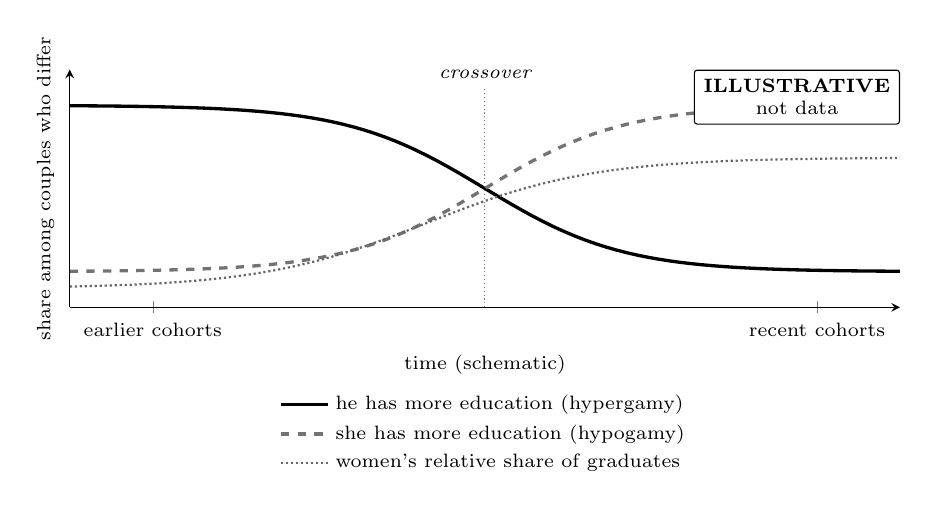
\begin{tikzpicture}
\begin{axis}[
  width=\columnwidth, height=4.6cm,
  xmin=0, xmax=10, ymin=0, ymax=1,
  xtick={1,9}, xticklabels={earlier cohorts, recent cohorts},
  ytick=\empty,
  xlabel={time (schematic)}, ylabel={share among couples who differ},
  ylabel style={font=\scriptsize}, xlabel style={font=\scriptsize},
  ticklabel style={font=\scriptsize},
  axis lines=left, clip=false,
  legend style={font=\scriptsize, draw=none, at={(0.5,-0.32)}, anchor=north, cells={anchor=west}},
  legend cell align=left,
]
\addplot[black, very thick, domain=0:10, samples=80] {0.15 + 0.7/(1+exp(1.2*(x-5)))};
\addlegendentry{he has more education (hypergamy)}
\addplot[black!55, very thick, dashed, domain=0:10, samples=80] {0.15 + 0.7/(1+exp(-1.2*(x-5)))};
\addlegendentry{she has more education (hypogamy)}
\addplot[black!60, densely dotted, thick, domain=0:10, samples=80] {0.08 + 0.55/(1+exp(-1.0*(x-4.3)))};
\addlegendentry{women's relative share of graduates}
\draw[black!50, densely dotted] (axis cs:5,0) -- (axis cs:5,0.92);
\node[font=\scriptsize\itshape, align=center, anchor=south] at (axis cs:5,0.92) {crossover};
\node[font=\scriptsize, draw, fill=white, rounded corners=1pt, anchor=north east, align=center]
  at (axis cs:10,1.0) {\textbf{ILLUSTRATIVE}\\not data};
\end{axis}
\end{tikzpicture}
